\documentclass[12pt]{article}
\usepackage{geometry}
\geometry{left=1in,right=0.75in,top=1in,bottom=1in}
\newcommand{\Problem}{E}
\newcommand{\Team}{2523245}
\usepackage{newtxtext}
\usepackage{amsmath,amssymb,amsthm}
\usepackage{newtxmath} % must come after amsXXX
\usepackage[pdftex]{graphicx}
\usepackage{xcolor}
\usepackage{fancyhdr}
\usepackage{booktabs}
\usepackage{subcaption}
\usepackage{caption}
\lhead{Team \Team}
\rhead{}
\cfoot{}
\newtheorem{theorem}{Theorem}
\newtheorem{corollary}[theorem]{Corollary}
\newtheorem{lemma}[theorem]{Lemma}
\newtheorem{definition}{Definition}
\captionsetup{skip=0.05cm}
\begin{document}
\graphicspath{{.}}  % Place your graphic files in the same directory as your main document
\DeclareGraphicsExtensions{.pdf, .jpg, .tif, .png}
\thispagestyle{empty}
\vspace*{-16ex}
\centerline{\begin{tabular}{*3{c}}
	\parbox[t]{0.3\linewidth}{\begin{center}\textbf{Problem Chosen}\\ \Large \textcolor{red}{\Problem}\end{center}}
	& \parbox[t]{0.3\linewidth}{\begin{center}\textbf{2025\\ ICM\\ Summary Sheet}\end{center}}
	& \parbox[t]{0.3\linewidth}{\begin{center}\textbf{Team Control Number}\\ \Large \textcolor{red}{\Team}\end{center}}	\\
	\hline
\end{tabular}}
%%%%%%%%%%%%%%% 环境配置结束 %%%%%%%%





%%%%%%%%%%% Summary开始 %%%%%%%%%%%
\setcounter{page}{1}



%%%%%%%%%%% Summary结束 %%%%%%%%%%%
%%%%%%%%%%%% 生成目录 %%%%%%%%%%%%
\clearpage
\pagestyle{fancy}
\tableofcontents 
\newpage
\rhead{Page \thepage\ }
%%%%%%%%%%% 生成目录结束 %%%%%%%%%%%%%
%%%%%%%%%% 正文开始 %%%%%%%%%%%%%%
\section{Introduction}

\section{Assumptions and Justifications}
\section{Notations}
\begin{table}[h]
	\centering
	\begin{tabular}{cc}
	\toprule[2pt]
		\textbf{Notations} & \textbf{Explanations} \\
	\midrule[1pt]
	$LSR$ & Loss of Species Richness (\%) \\
	$TES$ & Total Ecosystem Stability \\
	\bottomrule[2pt]
	\end{tabular}
\end{table}


\section{Food Web Model}
\hspace{2em}Food webs are sophisticated. Before humans get involved, however, a majority of ecosystems evolve in their exclusive dynamics. Noticing such characteristic of nature, we separate the food web into two sub-models. 

Firstly, We propose the Elementary Ecology Interaction Model (EEIM) to simulate natural processes of ecosystem evolution excluding human factors (e.g., chemical pollution). Then we design the Elementary Ecology Destroyer Model (EEDM) to introduce human interference, particularly chemicals overuse, into ecosystem evolution. Finally, the Food Web Model is established by integrating EEIM and EEDM, which comprehensively and accurately interpret the evolution dynamics of forest-to-farm agricultural ecosystems.
\subsection{Basic Food Web Model}
\subsection{Elementary Ecology Destroyer Model, EEDM.}
\hspace{2em}In section 4.1, we propose the EEIM to model the food web under an ideal circumstance where chemical substances are excluded. In this chapter, we introduce the Elementary Ecology Destroyer Model (EEDM) to encompass humans' overuse of chemicals and corresponding negative effects on agricultural ecosystems. The final food web model which takes all the factors into consideration is made up of EEDM and EEIM.
% 数据集构造思路
\begin{figure}[h]
	\centering
	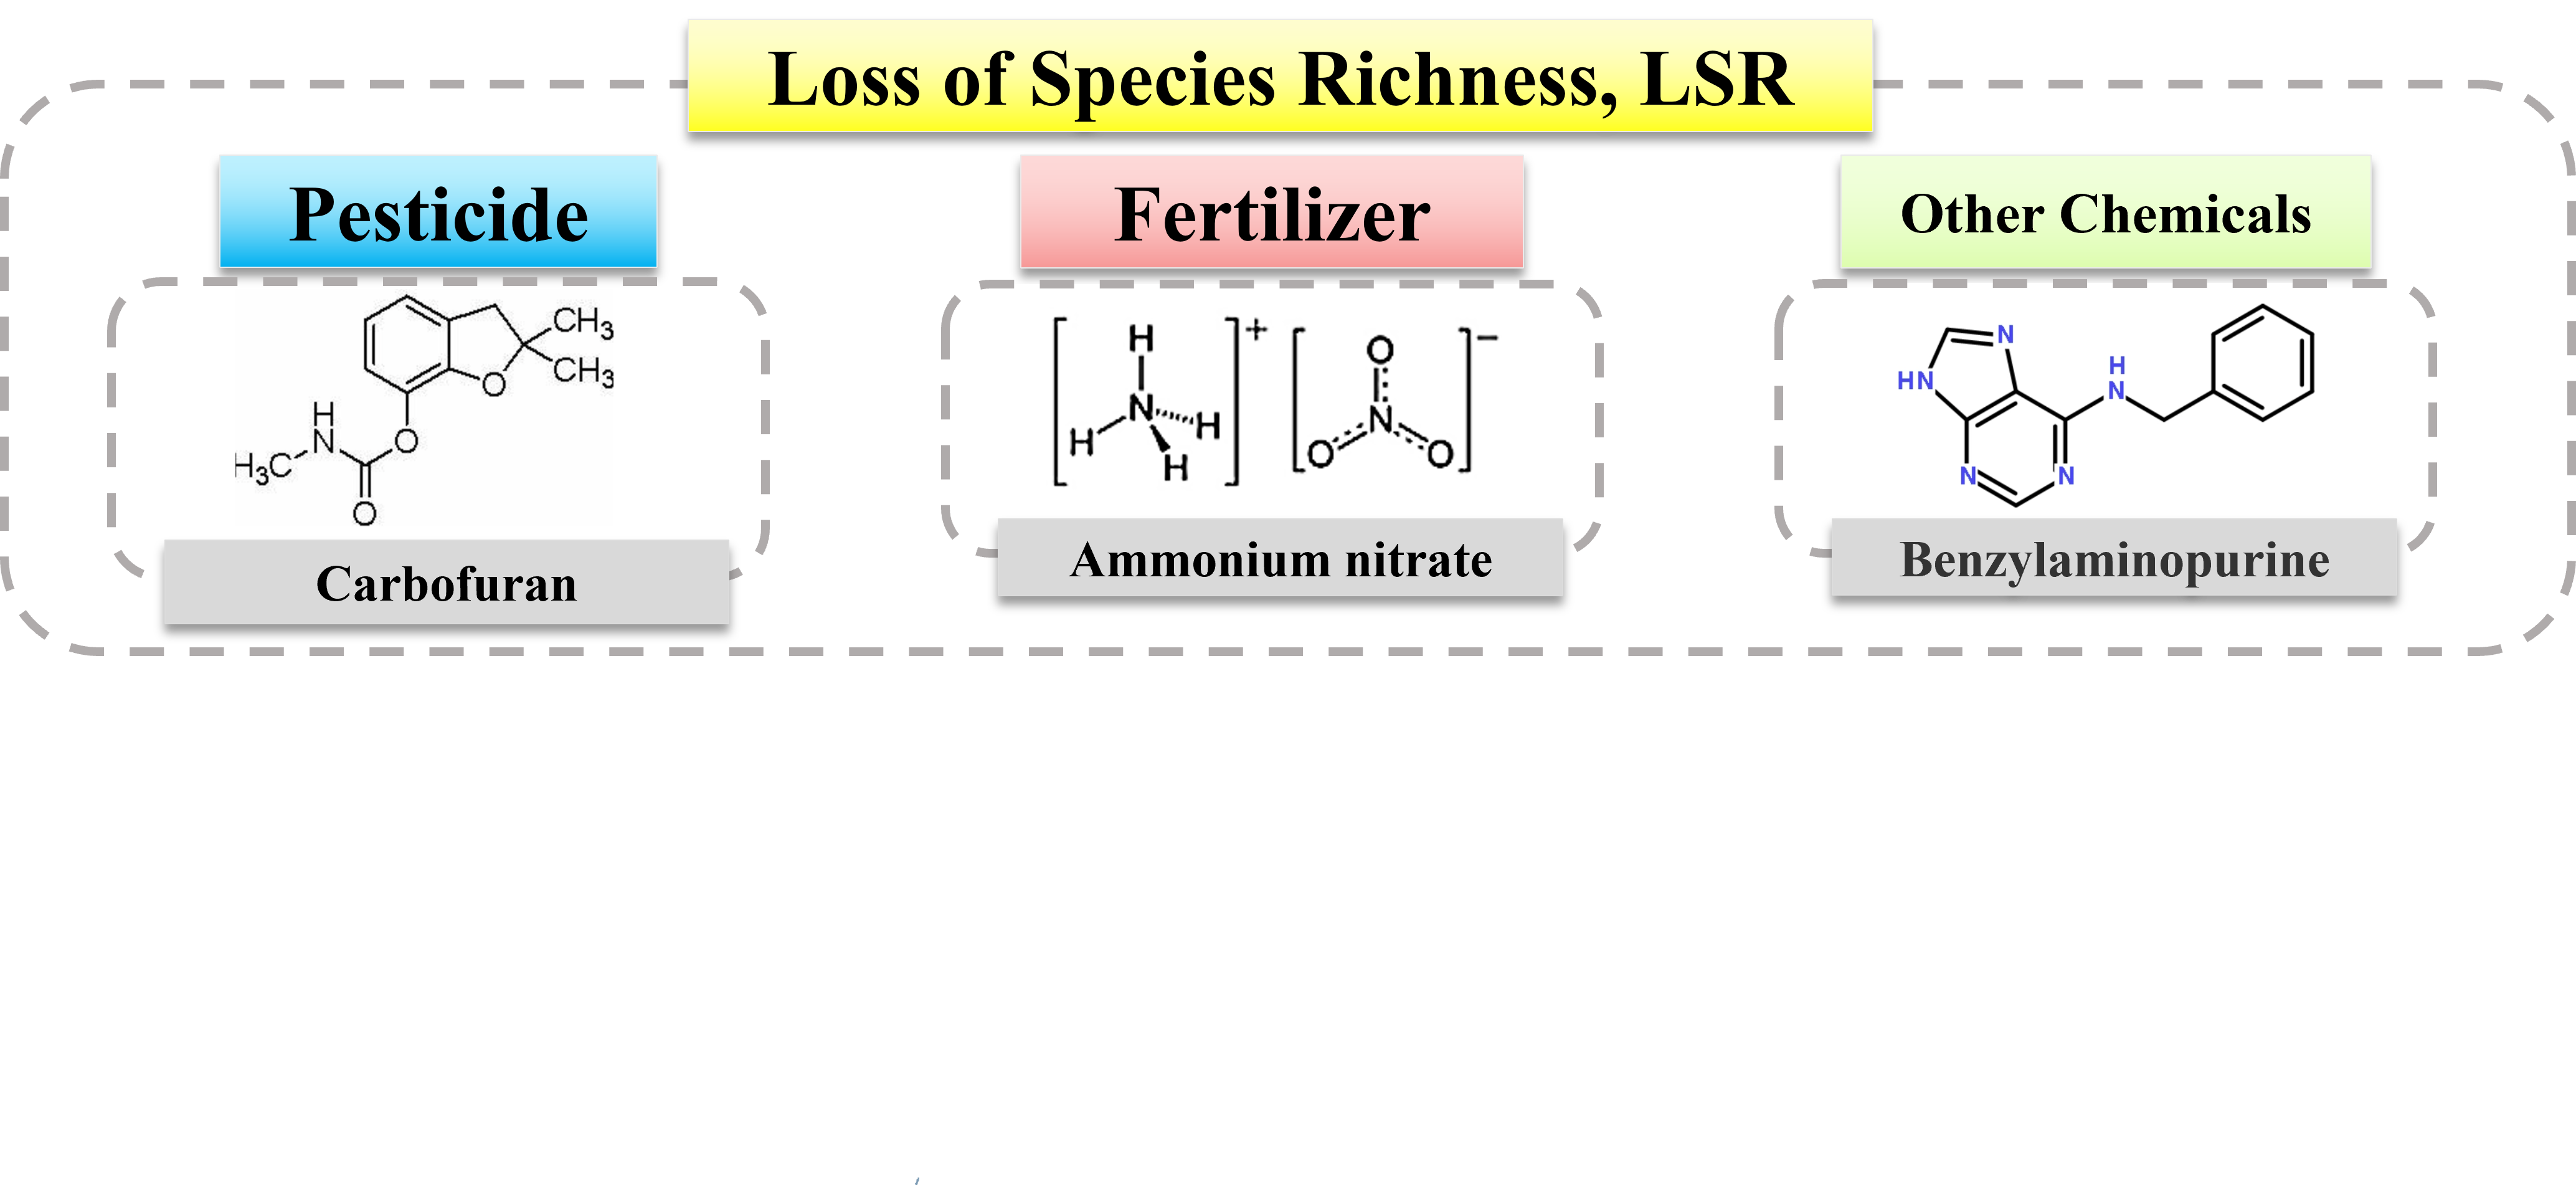
\includegraphics[width=0.5\textwidth]{./figures/dataset.png}
	\caption{Selected variables for the training dataset.}
	\label{dataset.}
\end{figure}
Numerous relevant researches have observed the over-complicated relationship between chemical usages and their corresponding effects. To simplify the process, we employ deep-learning methods, to be specific, the Multi-Layer-Perceptron (MLP) to better quantify the relationship between pivotal parameters and the loss of species richness. We follow a rigorous procedure to train our neural network, from dataset-preparation to robustness evaluation.


\textbf{Dataset Preparation. }Usages of pesticides ($Pest.$), fertilizers ($Fert.$) and other chemicals ($Oths.$) are selected to be the input features, considering they are the major categories of contemporary agricultural chemicals. Loss of species richness ($LSR$) is chosen as the output label, as is illustrated in figure \ref{dataset.}. All the datas are collected from \cite{1}\cite{2}\cite{3}.

% MLP的构造思路
\begin{figure}[h]
	\centering
	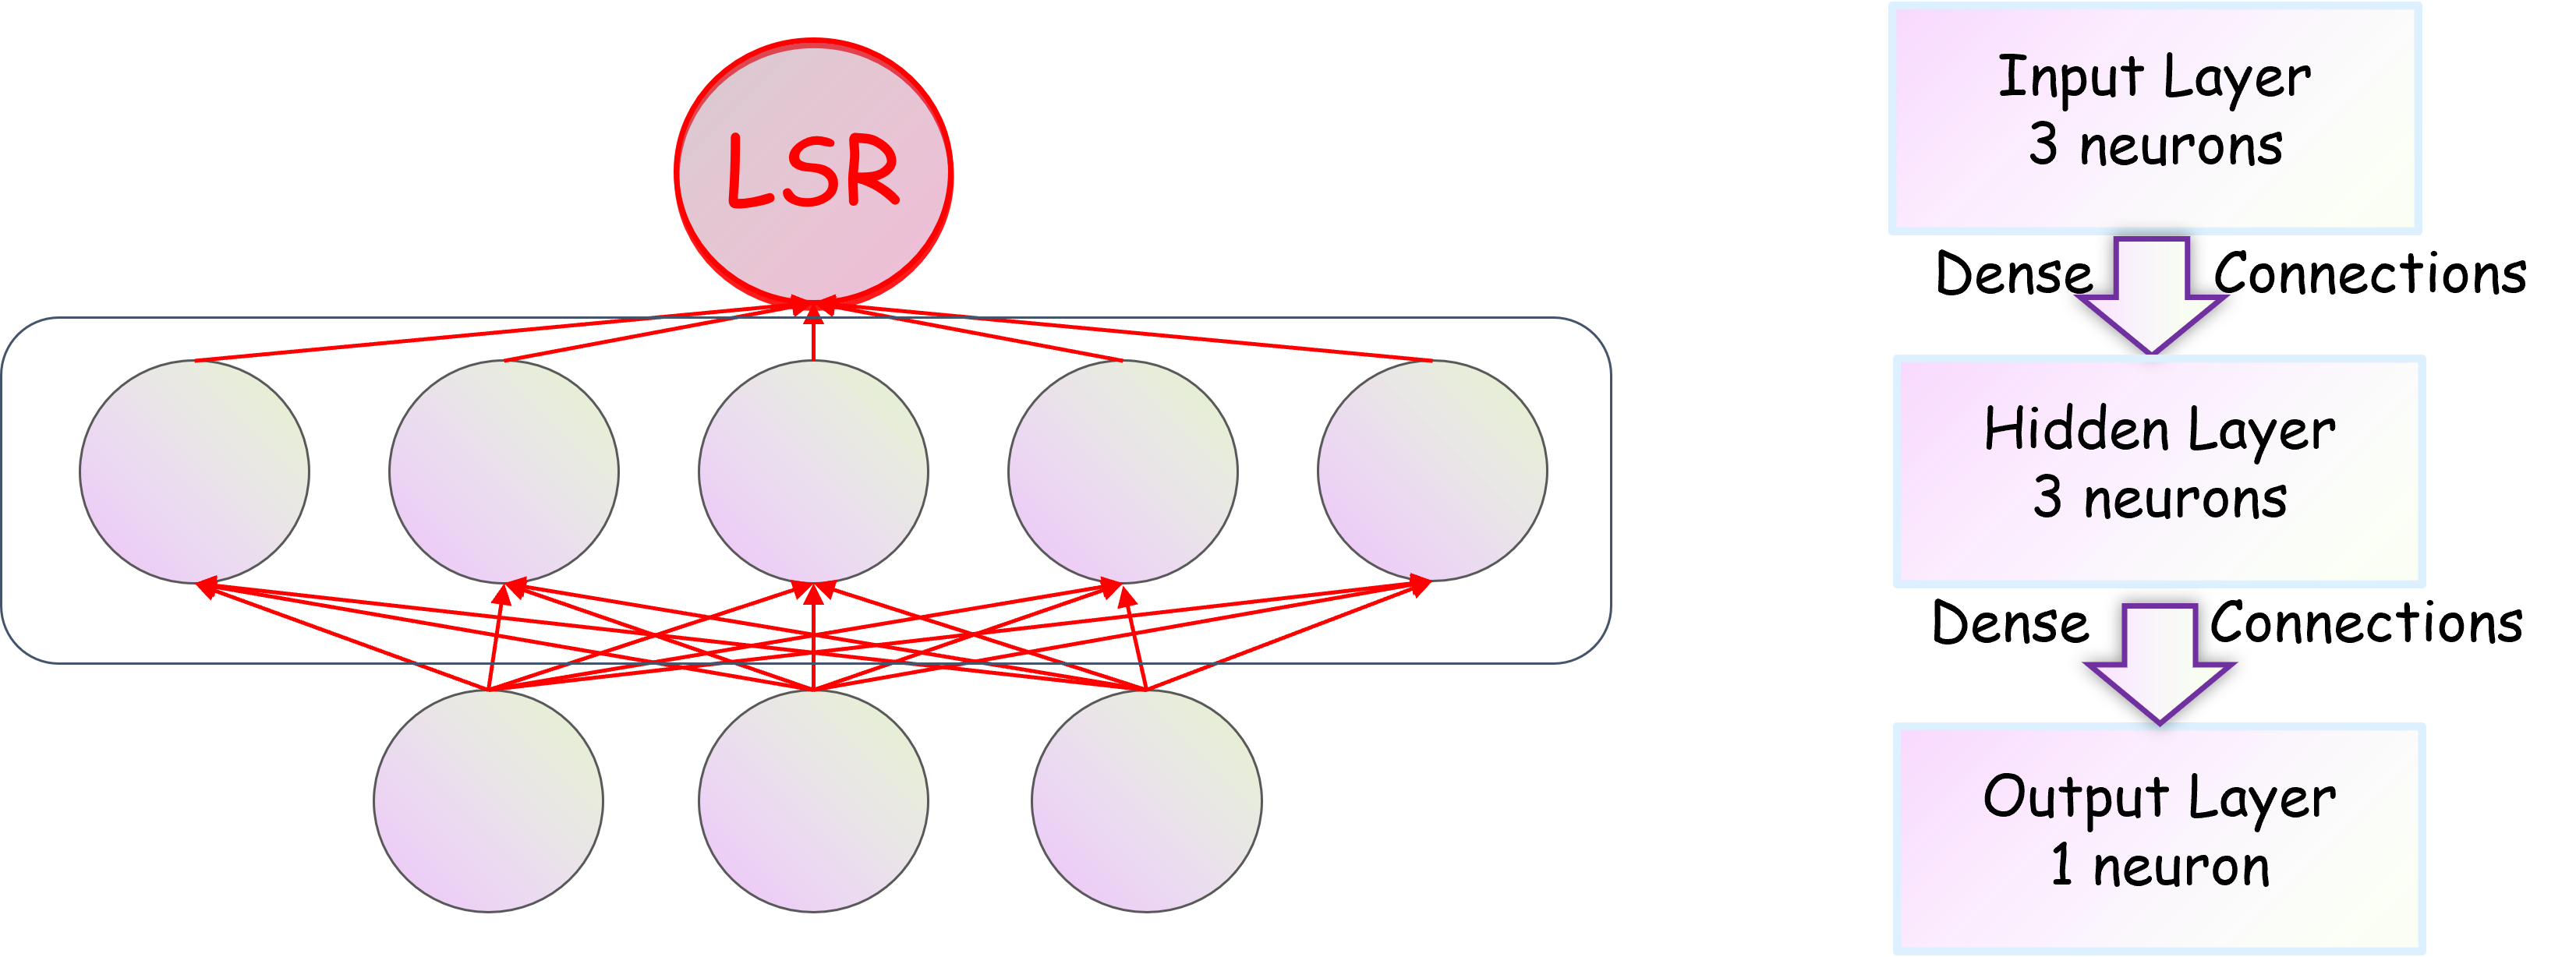
\includegraphics[width=0.6\textwidth]{./figures/MLP.png}
	\caption{Backbone MLP structure of the EEDM.}
	\label{MLP}
\end{figure}

\textbf{Experimental Configuration. }We applied one RTX 4060 GPU as hardware platform and the PyTorch Deep-Learning Framework. Mean Squared Loss (MSE) and Small Gradient Descents (SGD) are chosen respectively as loss function and optimization algorithm, as is shown in equation \ref{optimization}. Hyper-parameters are configured as: $batch\_size=16,\ epochs=1000,\ learning\_rate=0.001$. Additionally, regularization techniques are employed to mitigate over-fitting: $dropout\_ratio=0.2$. Finally, we designed a 3-3-1 neuron distribution for MLP (figure \ref{MLP}), which could be expressed as equation \ref{fp}, where $\textbf{W}_1\in\mathbb{R}^{3\times3},\textbf{W}_2\in\mathbb{R}^{1\times3},\textbf{b}_1\in\mathbb{R}^{3\times1},\textbf{b}_2\in\mathbb{R}^{1\times1},\sigma(\cdot)\in\mathbb{R}^{3\times3}$

% 损失函数和优化算法
\begin{equation}
	L(\textbf{w},b)=\frac{1}{n}\sum_{i=1}^{\mathbb{B}}\frac{1}{2}(\textbf{w}^T\textbf{x}^{(i)}+b-y^{(i)})^2,\hspace{0.3em}(\textbf{w},b)\leftarrow(\textbf{w},b)-\frac{\eta}{|\mathcal{B}|}\sum_{i\in\mathcal{B}}\partial_{(\textbf{w},b)}l^{(i)}(\textbf{w},b).
	\label{optimization}
\end{equation}

% MLP基本原理
\begin{equation}
	\begin{cases}
		\textbf{O} = \sigma(\textbf{W}_1\cdot\textbf{X}+\textbf{b}) \\
		LSR = \textbf{W}_2\cdot\textbf{O} + \textbf{b}
	\end{cases},\hspace{0.2em}\text{where}\hspace{0.2em}\sigma(\cdot)=\mathrm{ReLU(\cdot)}
	\label{fp}
\end{equation}

We further processed equation \ref{fp} to transform it linearly, which goes as:
\begin{equation}
	LSR = \textbf{W}_{total}\cdot\textbf{X}+b_{total},\hspace{0.2em}\text{where}\hspace{0.2em}\begin{cases}
		\textbf{W}_{total} = \textbf{W}_2\cdot\sigma(x_i)\cdot\textbf{W}_1 \\
		\textbf{b}_{total} = \textbf{W}_2\cdot\sigma(x_i)\cdot\textbf{b}_1 + \textbf{b}_2
	\end{cases}
\end{equation}

Through training (figure \ref{t}) we acquire the primitive form of EEDM:
\begin{align}
	& \begin{cases}
	\textbf{W}_{total} = \begin{pmatrix}
	-0.263 \\ 0.273 \\ -0.288
\end{pmatrix}^{\top}\cdot\begin{pmatrix}
	1 & 0 & 0 \\
	0 & 1 & 0 \\
	0 & 0 & 1
\end{pmatrix}\cdot\begin{pmatrix}
	-0.295 & -0.281 & -0.322 \\
	0.307 & 0.263 & 0.323 \\
	-0.282 & -0.258 & -0.310
\end{pmatrix}=\begin{pmatrix}
	0.243 \\ 0.220 \\ 0.262
\end{pmatrix}^{\top} \\
\textbf{b}_{total} = \begin{pmatrix}
	-0.263 \\ 0.273 \\ -0.288
\end{pmatrix}^{\top}\cdot\begin{pmatrix}
	1 & 0 & 0 \\
	0 & 1 & 0 \\
	0 & 0 & 1
\end{pmatrix}\cdot\begin{pmatrix}
-0.174 \\ 0.179 \\ -0.167
\end{pmatrix}+(0.103) = 0.246
	\end{cases} \\
	& \xrightarrow{}LSR(\%) = 0.243\times Pest.(kg/ha) + 0.220\times Fert.(kg/ha) + 0.262\times Oths.(kg/ha) + 0.246
	\label{primitive}
\end{align}
where $LSR$ if the loss of species richness, $Pest.$, $Fert.$, $Oths.$ respectively stands for the quantity of used pesticides, fertilizers and other chemicals.
% 训练图
\begin{figure}[htbp]
	\centering
	\begin{subfigure}{0.35\textwidth}
		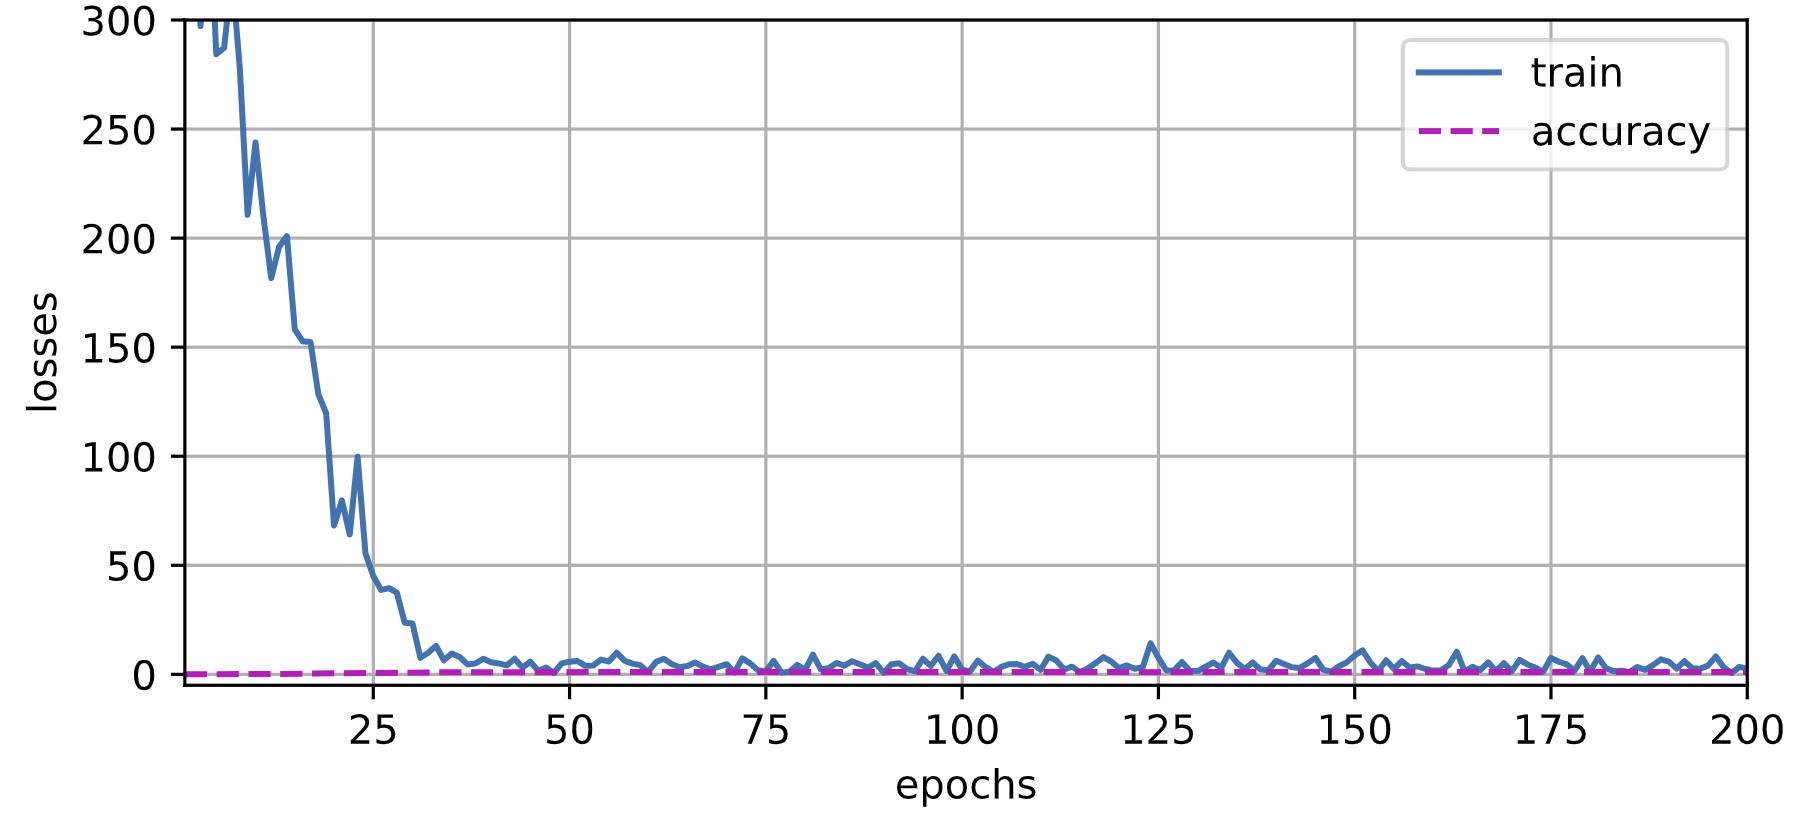
\includegraphics[width=\textwidth]{./figures/train.png}
		\label{train}
	\end{subfigure}
	\begin{subfigure}{0.35\textwidth}
		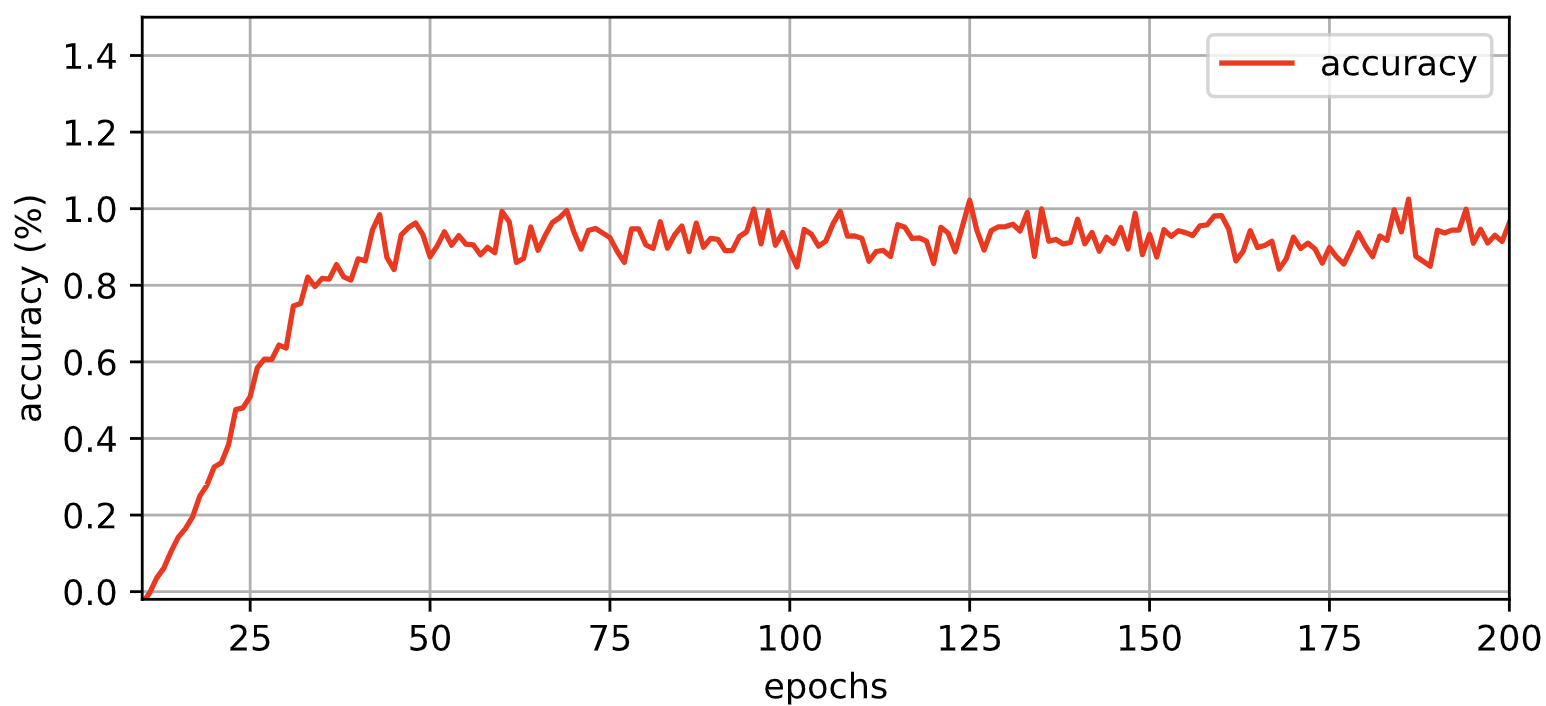
\includegraphics[width=\textwidth]{./figures/accuracy.png}
		\label{test}
	\end{subfigure}
	\caption{Our model-training process.}
	\label{t}
\end{figure}

A deeper optimization is conducted by mapping EEDM (equation \ref{primitive}) to time-dimension. Considering each of its sub-variables as functions correlated to time, we use \textbf{MATLAB} to fit each equation, culminating in a time-based EEDM (equation \ref{time}, figure \ref{ti}):
\begin{align}
	&LSR = \begin{pmatrix}
		\alpha(t) \\ \beta(t) \\ \theta(t)
	\end{pmatrix}=
	\begin{pmatrix}
		-0.0012619\times t^2+5.1116424\times t-5176.717 \\
		-0.06358907\times t^2+257.34633611\times t-260251.460 \\
		-0.001238\times t^2+5.02035714\times t-5087.3170
	\end{pmatrix} \\
	& \xrightarrow{ }LSR = -0.01462044487\times t^2+59.17365663\times t-59845.89449
	\label{time}
\end{align}

\begin{figure}[h]
	\centering
	\begin{subfigure}{0.3\textwidth}
	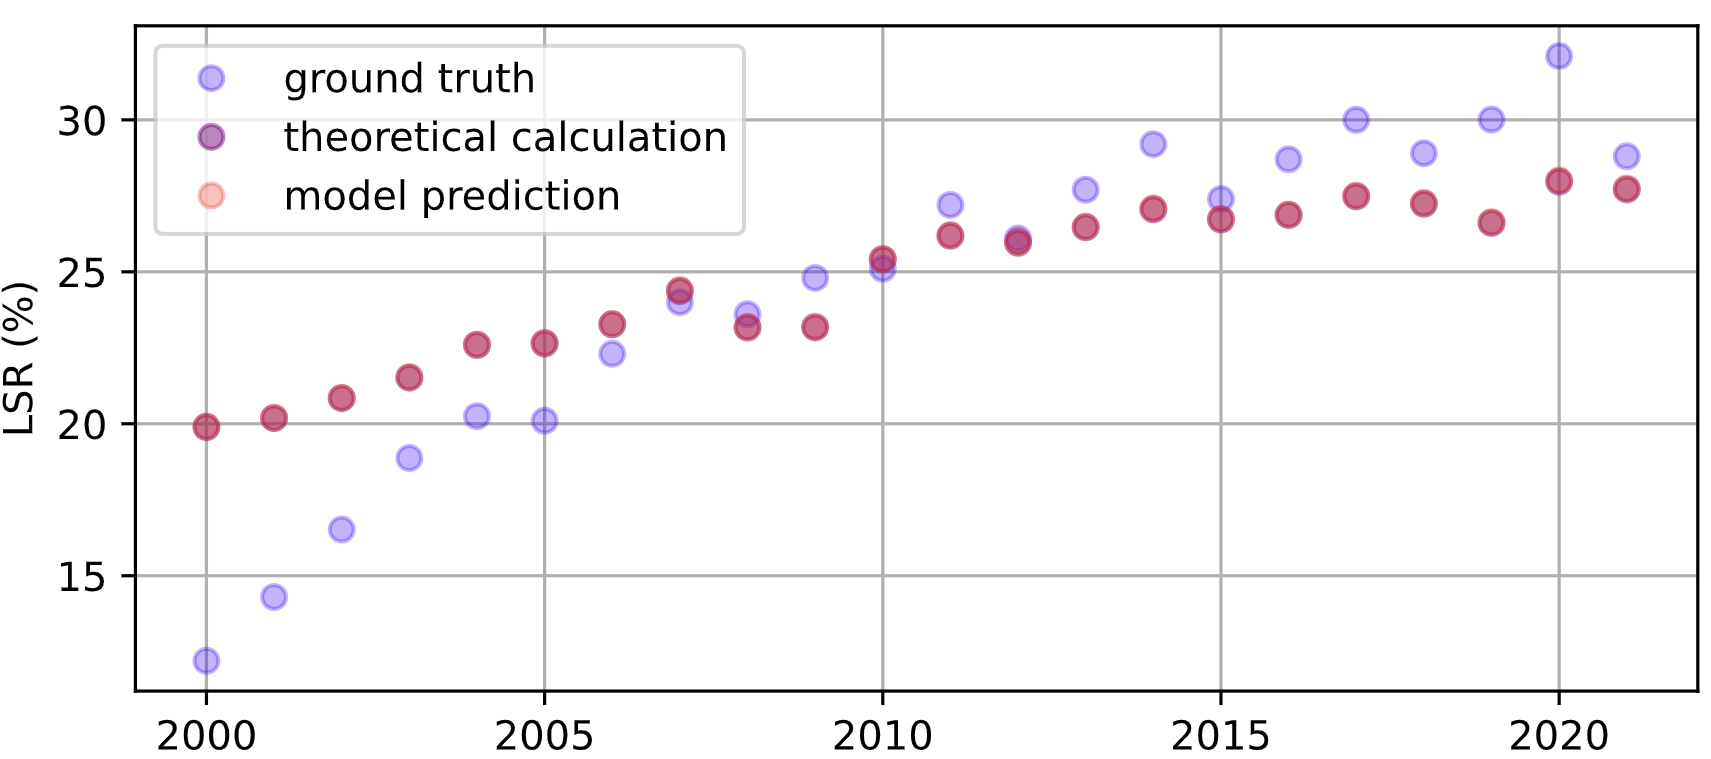
\includegraphics[width=\textwidth]{./figures/LSR_primitive_dimension.png}
\caption{Primitive Form.}
	\end{subfigure}
	\begin{subfigure}{0.3\textwidth}
		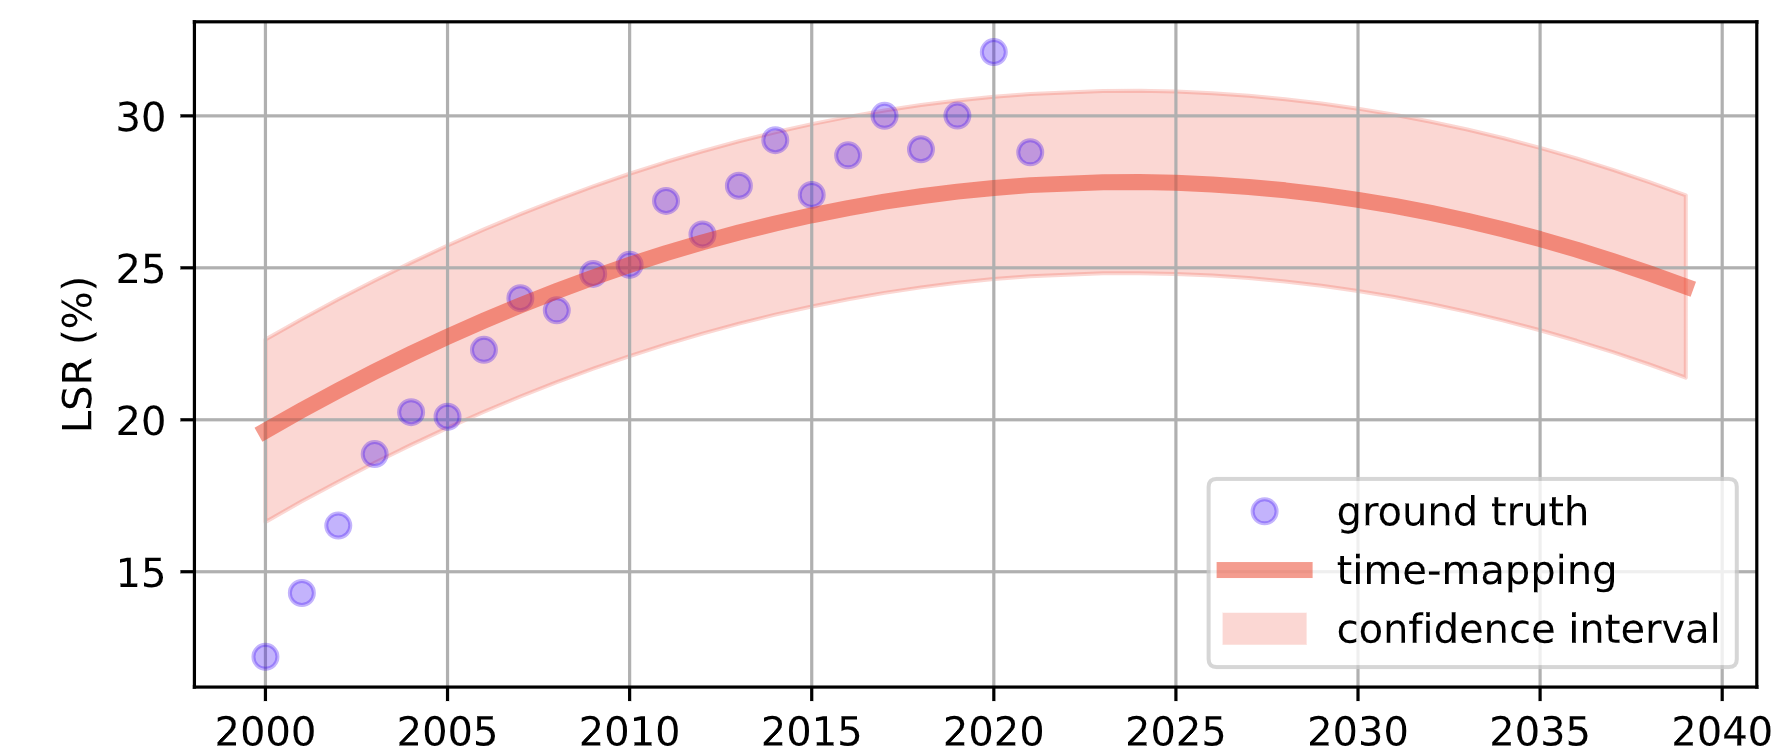
\includegraphics[width=\textwidth]{./figures/LSR_time_dimension.png}
		\caption{Time-dimension Form}
	\end{subfigure}
	\caption{Two forms of the EEDM: primitive and time-based respectively.}
	\label{ti}
\end{figure}

From figure \ref{t} it can be observed that our model reaches an accuracy of 90.3\%. We further validated our model by measuring the specific effects of chemical usages on birds population and the insects counterparts, as is illustrated in figure \ref{chemics}. It can be seen that overuse of chemicals contributes the greatest losses in plants richness, followed by insects. Such prediction aligns with reality since plants are the dominant creatures in agricultural ecosystems and insects are essential pollinators for crops.

\begin{figure}[h]
	\centering
	\begin{subfigure}[b]{0.43\textwidth}
		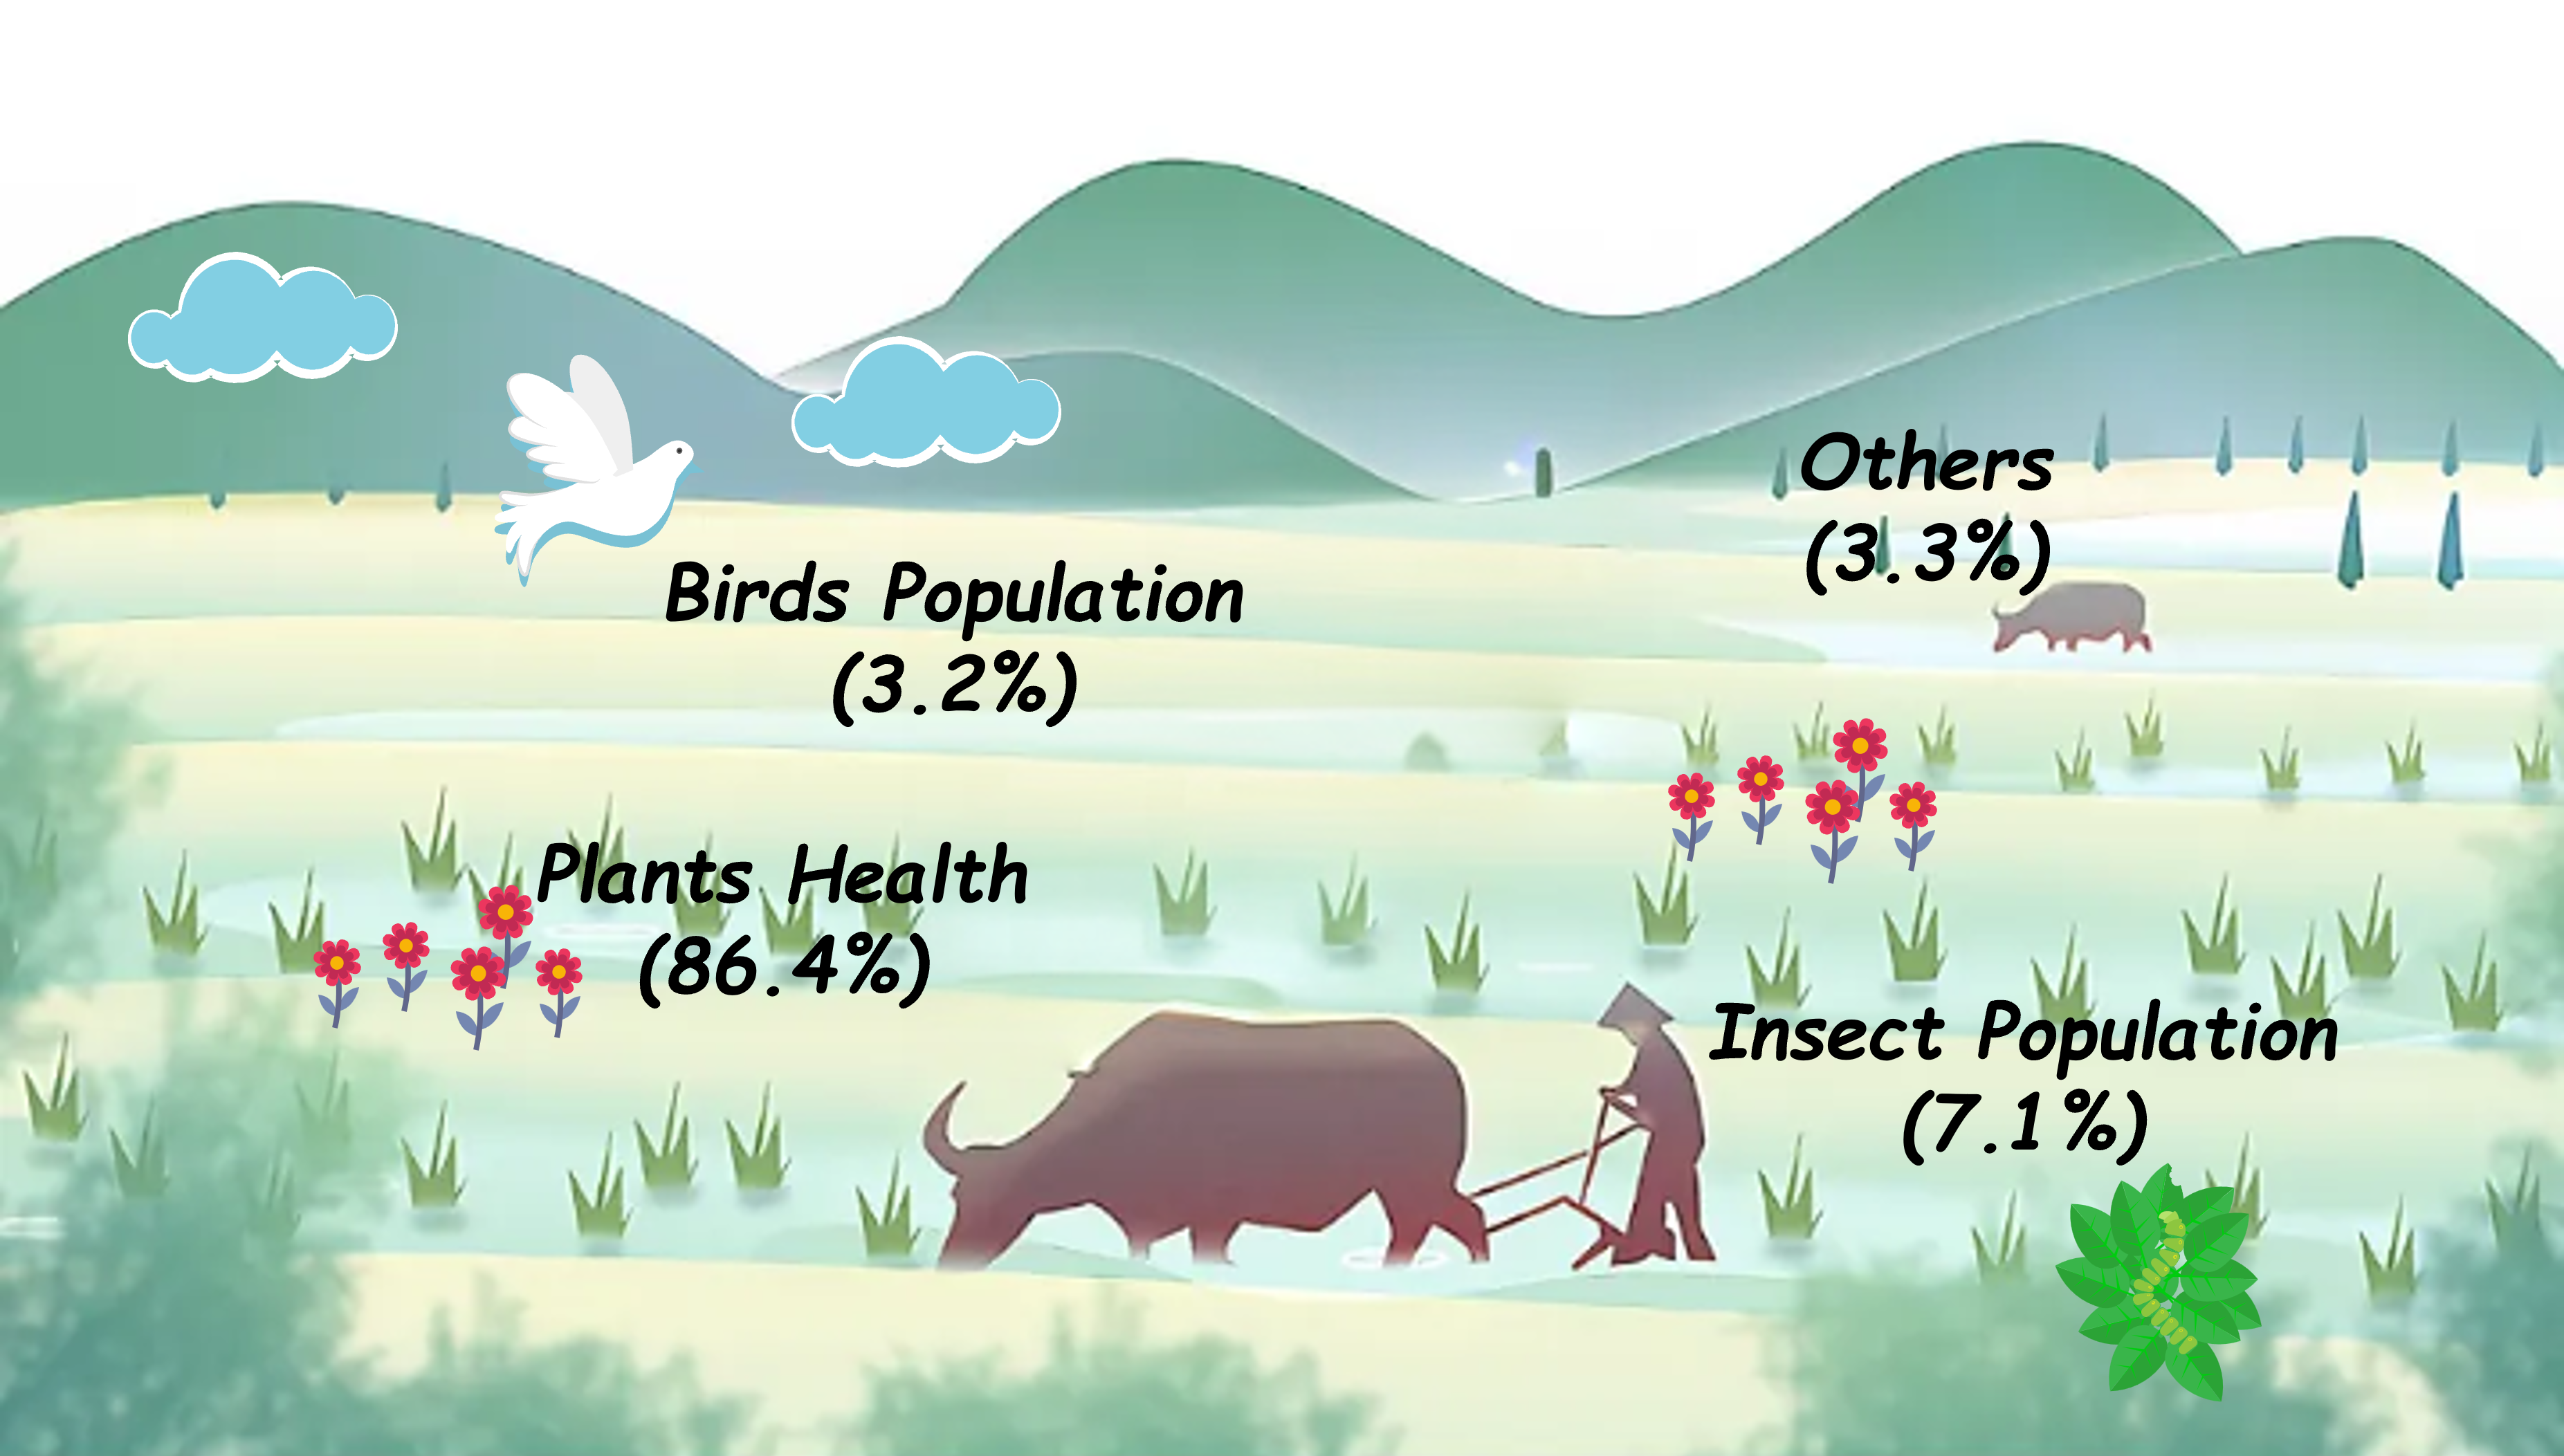
\includegraphics[width=\textwidth]{./figures/chemics on eco(task 1).png}
		\caption{Agricultural ecosystem.}
	\end{subfigure}
	\begin{subfigure}[b]{0.36\textwidth}
		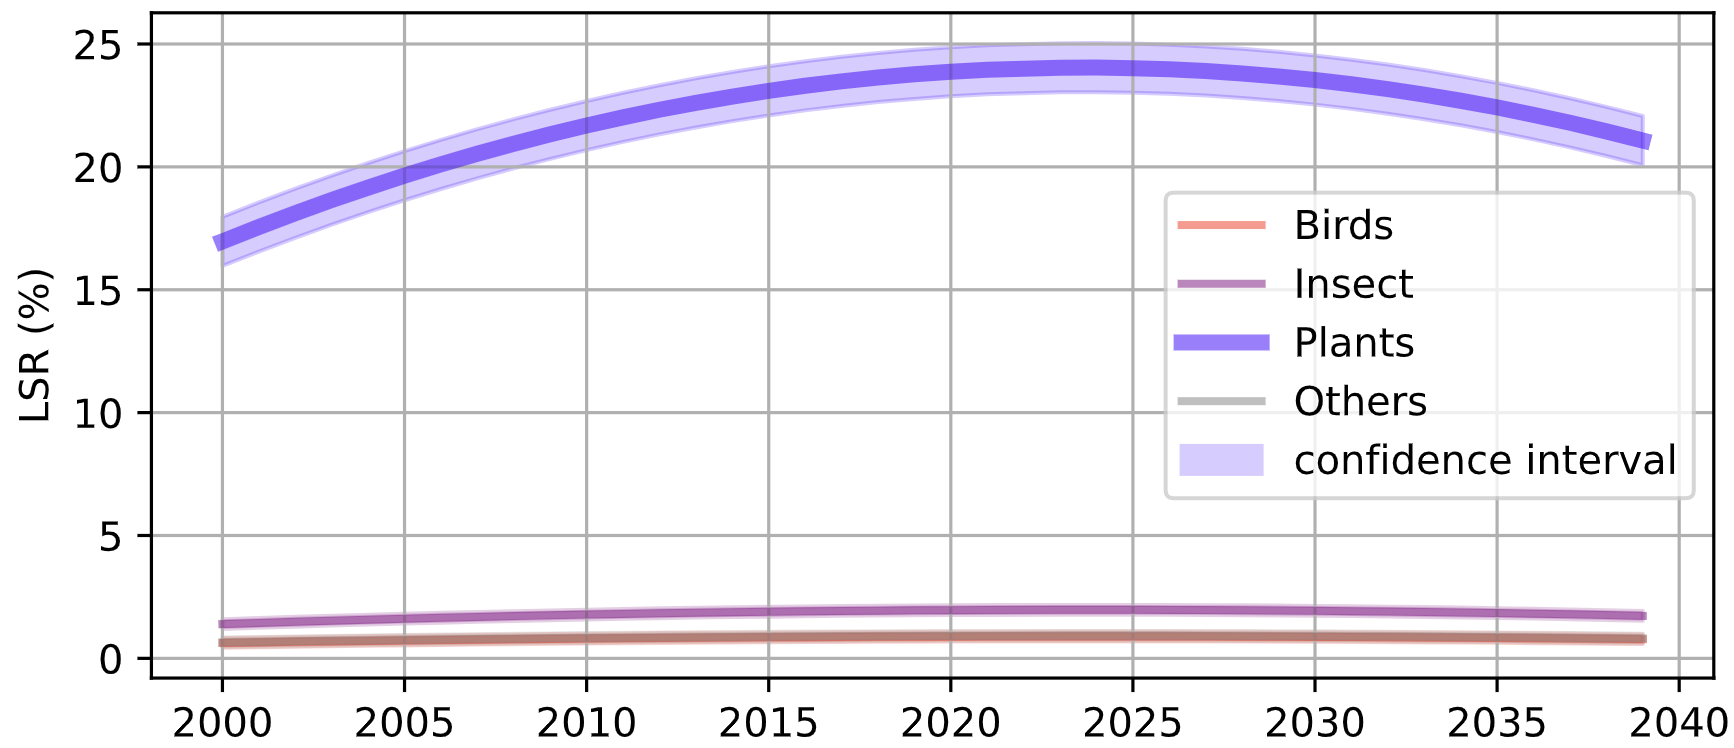
\includegraphics[width=\textwidth]{./figures/impacts_on_birds_etc(task 1)}
		\caption{Loss of species richness.}
	\end{subfigure}
	\caption{Effects of chemical usages on agricultural ecosystems.}
	\label{chemics}
\end{figure}

\subsection{Food Web Model}
\hspace{2em}By combining EEIM and EEDM into an integrated whole, we acquire the Food Web Model. Both sub-models exhibit dimensional consistency in calculated quantity while the mere difference lies in that EEIM calculates the species richness and EEDM the absolute value of losses on the counterparts. Existing researches(\cite{4}) have pointed out that ecosystem stability is proportional to species richness, so we define the Food Web Model as:\begin{equation}
	Food\ Web\ Model = EEIM - EEDM,\ \textbf{or}\ Stability/Richness=EEIM-EEDM
	\label{shiboqi_hetiban}
\end{equation}
where $Stability$ and $Richness$ is evaluated by a ratio regarding species biodiversity of unexploited regions as its baseline. From article \ref{5} we define ``unexploited regions'' as ``primary vegetation with low landscape cropland coverage and with minimal nitrogen fertilizer application rate.''

Food Web Model is visualized by integrating figure \ref{shiboqi} and \ref{ti} on time-dimension referring to equation \ref{shiboqi_hetiban}, as is illustrated in figure \ref{shiboqi_hetibian_detu}, where the shaded areas represent 95\% data confidence intervals and $Normalized\ Ratio$ stands for overall biodiversity and species richness percentage comparing to unexploited regions. Since the model takes all factors into consideration (e.g., pesticides, agricultural cycle, etc.), it comprehensively reflects the primitive evolution dynamics of agricultural ecosystems and to what extent of damage humans have caused to existing regions.
% 合体版示波器
\begin{figure}[h]
	\centering
	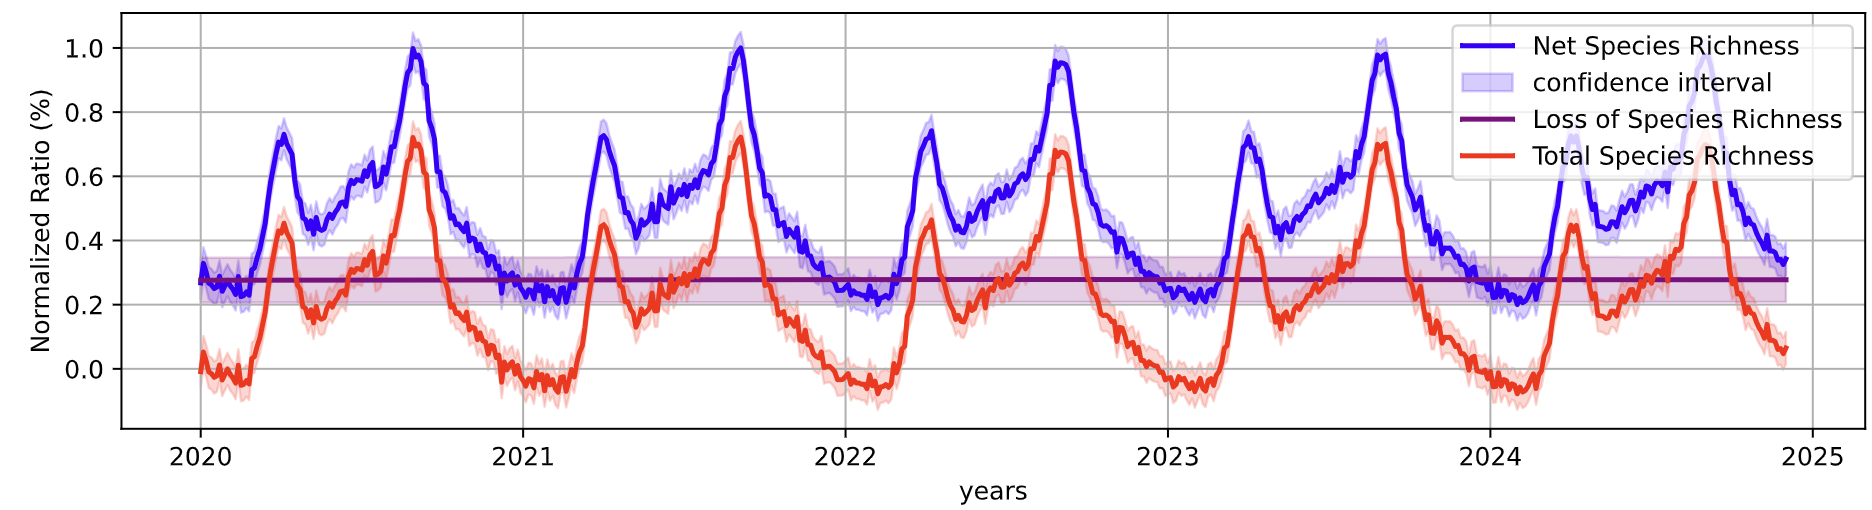
\includegraphics[width=0.9\textwidth]{./figures/shiboqi_hetiban(task1).png}
	\caption{Visualization of the Food Web Model.}
	\label{shiboqi_hetibian_detu}
\end{figure}



\section{Reemergence of native species---\textit{``They Are Home''}}
\hspace{2em}Edge habitats sit in the buffer zone between agricultural fields and surrounding ecosystems. Considering that our research focus is forest-to-farm situations, we assume the surrounding ecosystems are natural forests. In this section, we applied the broadened version of Pascal's Triangle and Ecosystem Stability Model to evaluate impacts of native species' reemergence, which offer a dynamic view on the complete process of ecosystem evolution.
\subsection{Pascal's Triangle is all you need}
\hspace{2em}Native species are considered to have migrated into edge habits due to human exploits on the primary evolution stage of agricultural ecosystems. Therefore, they feature strong seasonal dynamics and geographical movements.

Pascal's Triangle is a triangular array of number which is widely used in algebra. Notice that the shape follows an increasing trend from inside out, we utilize this characteristic to demonstrate the geographical distributions of native species in terms of diverse evolution stages. By concatenating two triangles together into a square, we have the broadened Pascal's Triangle, which goes as:
\begin{equation}
	\begin{matrix}
				& & & &1 & & & & \\
		& & &1&  &1& & & \\
		& &1& &2 & &1 & & \\
		&1& &3&  &3&  &1 & \\ 
		&1& &3&  &3&  &1 & \\ 
		& &1& &2 & &1 & & \\
		& & &1&  &1& & & \\
		& & & &1 & & & & \\
	\end{matrix}\hspace{0.2em} \iff\hspace{0.3em}C(n,k)_x=C(n,k)_y=\frac{n!}{k!(n-k)!}\iff\begin{pmatrix}
	C_x \\C_y
	\end{pmatrix}
\end{equation}

Similarly, by taking reciprocal on each value, we acquire another version of Pascal's Triangle which could be applied to explain the intermediate evolution periods when the majority of native species distribute in edge habitats: $\begin{pmatrix}
	\frac{1}{C_x} & \frac{1}{C_y}
\end{pmatrix}$. Visualization of both Pascal's Triangle is illustrated in figure \ref{tr}.
% 这是杨辉的两种形式
\begin{figure}[h]
	\centering
	\begin{subfigure}{0.25\textwidth}
		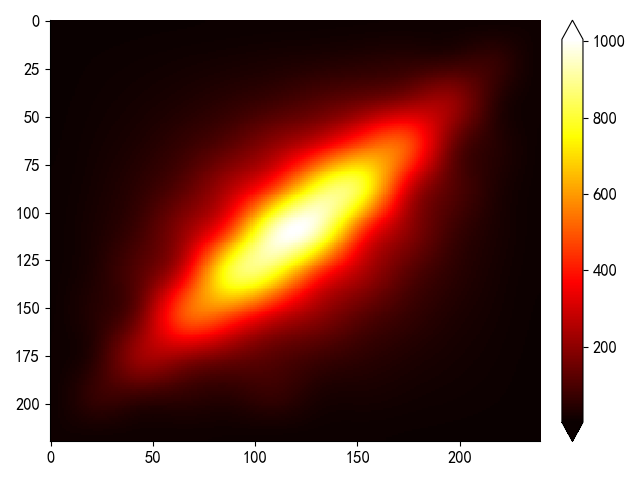
\includegraphics[width=\textwidth]{./figures/primitive triangle(task2).png}
		\caption{Primitive form.}
		\label{p}
	\end{subfigure}
	\begin{subfigure}{0.25\textwidth}
		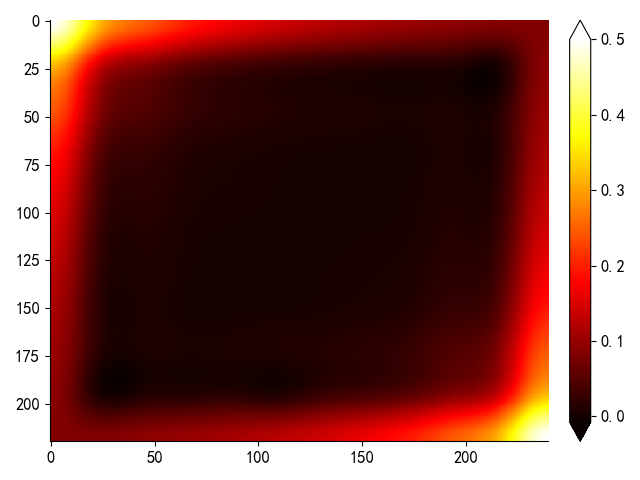
\includegraphics[width=\textwidth]{./figures/primitive reprocical triangle(task2)}
		\caption{Reciprocal form.}
		\label{wobuxaingxiele}
	\end{subfigure}
	\caption{Broadened Pascal's Triangle, where a brighter color indicates a larger species richness.}
	\label{tr}
\end{figure}

What differs \ref{p} and \ref{wobuxaingxiele} is their application scenarios. Figure \ref{p} describes the elementary stage of agricultural ecosystem evolution where the majority of native species distribute in central regions featuring sufficient living resources; Figure \ref{wobuxaingxiele} demonstrates the middle periods of evolution where the human exploits get involved and are transforming it into an agricultural ecosystem. Native species are accordingly compelled to migrate into edge habitats. 
\subsection{Impacts of reemergence of native species}
\hspace{2em}The migration process is firstly simulated using our Broadened Pascal's Triangle. It's worth noting that, instead of choosing two specific species, we select symbolic creatures of two categories, namely $A$ and $B$, to generalize our model. Species $A$ is a native insect featuring dense population (such as \textit{Apis Mellifera}) while $B$ is a local animal with long lifespan but relatively low population (such as \textit{Cervus Elaphus}). 

As is illustrated in figure \ref{mig}, the triple periods of ecosystem evolution are demonstrated, including stage 1 (Natural Forest Area), stage 2 (Converted Agricultural System) and stage 3 (Mature Ecosystem). In stage 1, $A$ and $B$ settle in central regions; In stage 2, they migrated into edge habitats temporarily to escape human interference,; In stage 3, due to a flourished and mature agricultural system, both species reemerged and relocated, sharing the living resources with human beings.
\begin{figure}[h]
	\centering
	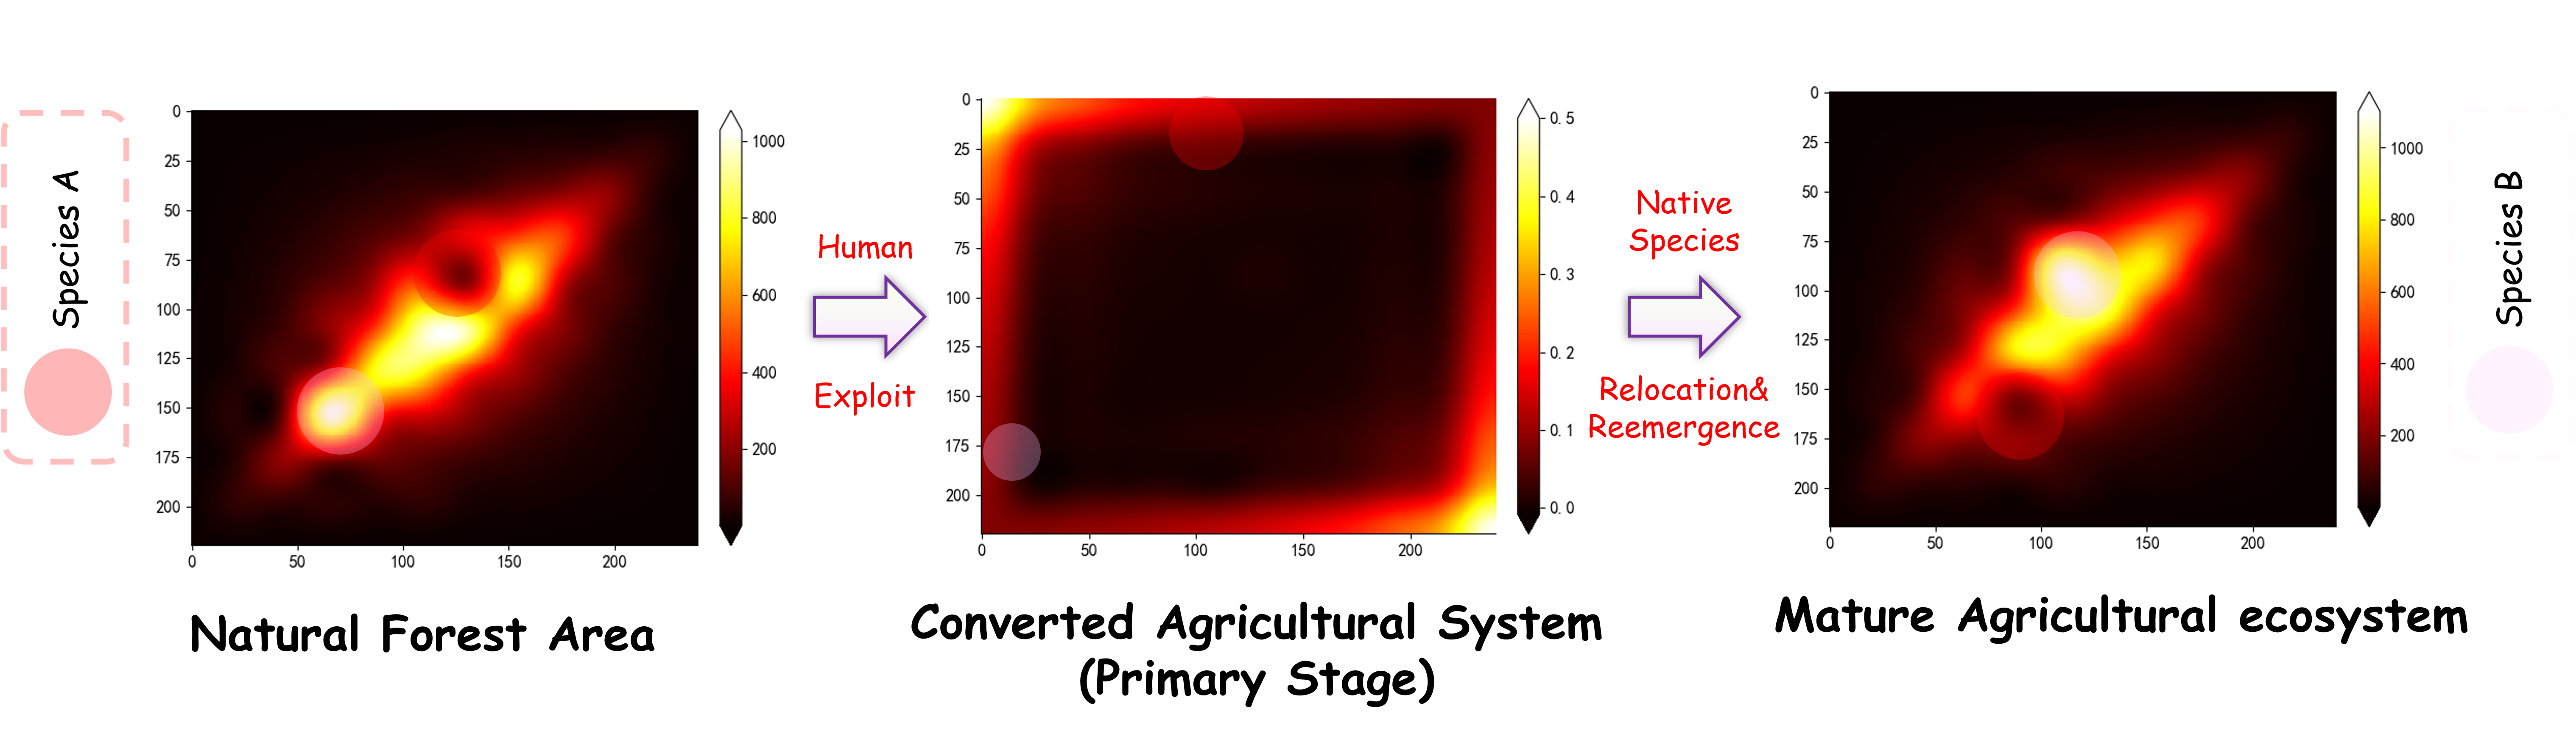
\includegraphics[width=\textwidth]{./figures/reemergence(task 2).png}
	\caption{Three stages in ecosystem evolution and native species' reemergence.}
	\label{mig}
\end{figure}

While the Broadened Pascal's Triangle describes the dynamic reemergence of native species, the Ecosystem Stability Model (ESM) reveals the exact influence of species' reemergence on overall ecosystem stability. 

ESM is composed of Resilience Stability ($RLS$) and Resistant Stability ($RTS$), both of which are correlated with species richness or diversity. Therefore, the reemergence of  $A$ and $B$ directly positively impacts the ecosystem by contributing to $RLS$ and $RTS$.

\begin{figure}[h]
	\centering
	\begin{subfigure}[b]{0.46\textwidth}
	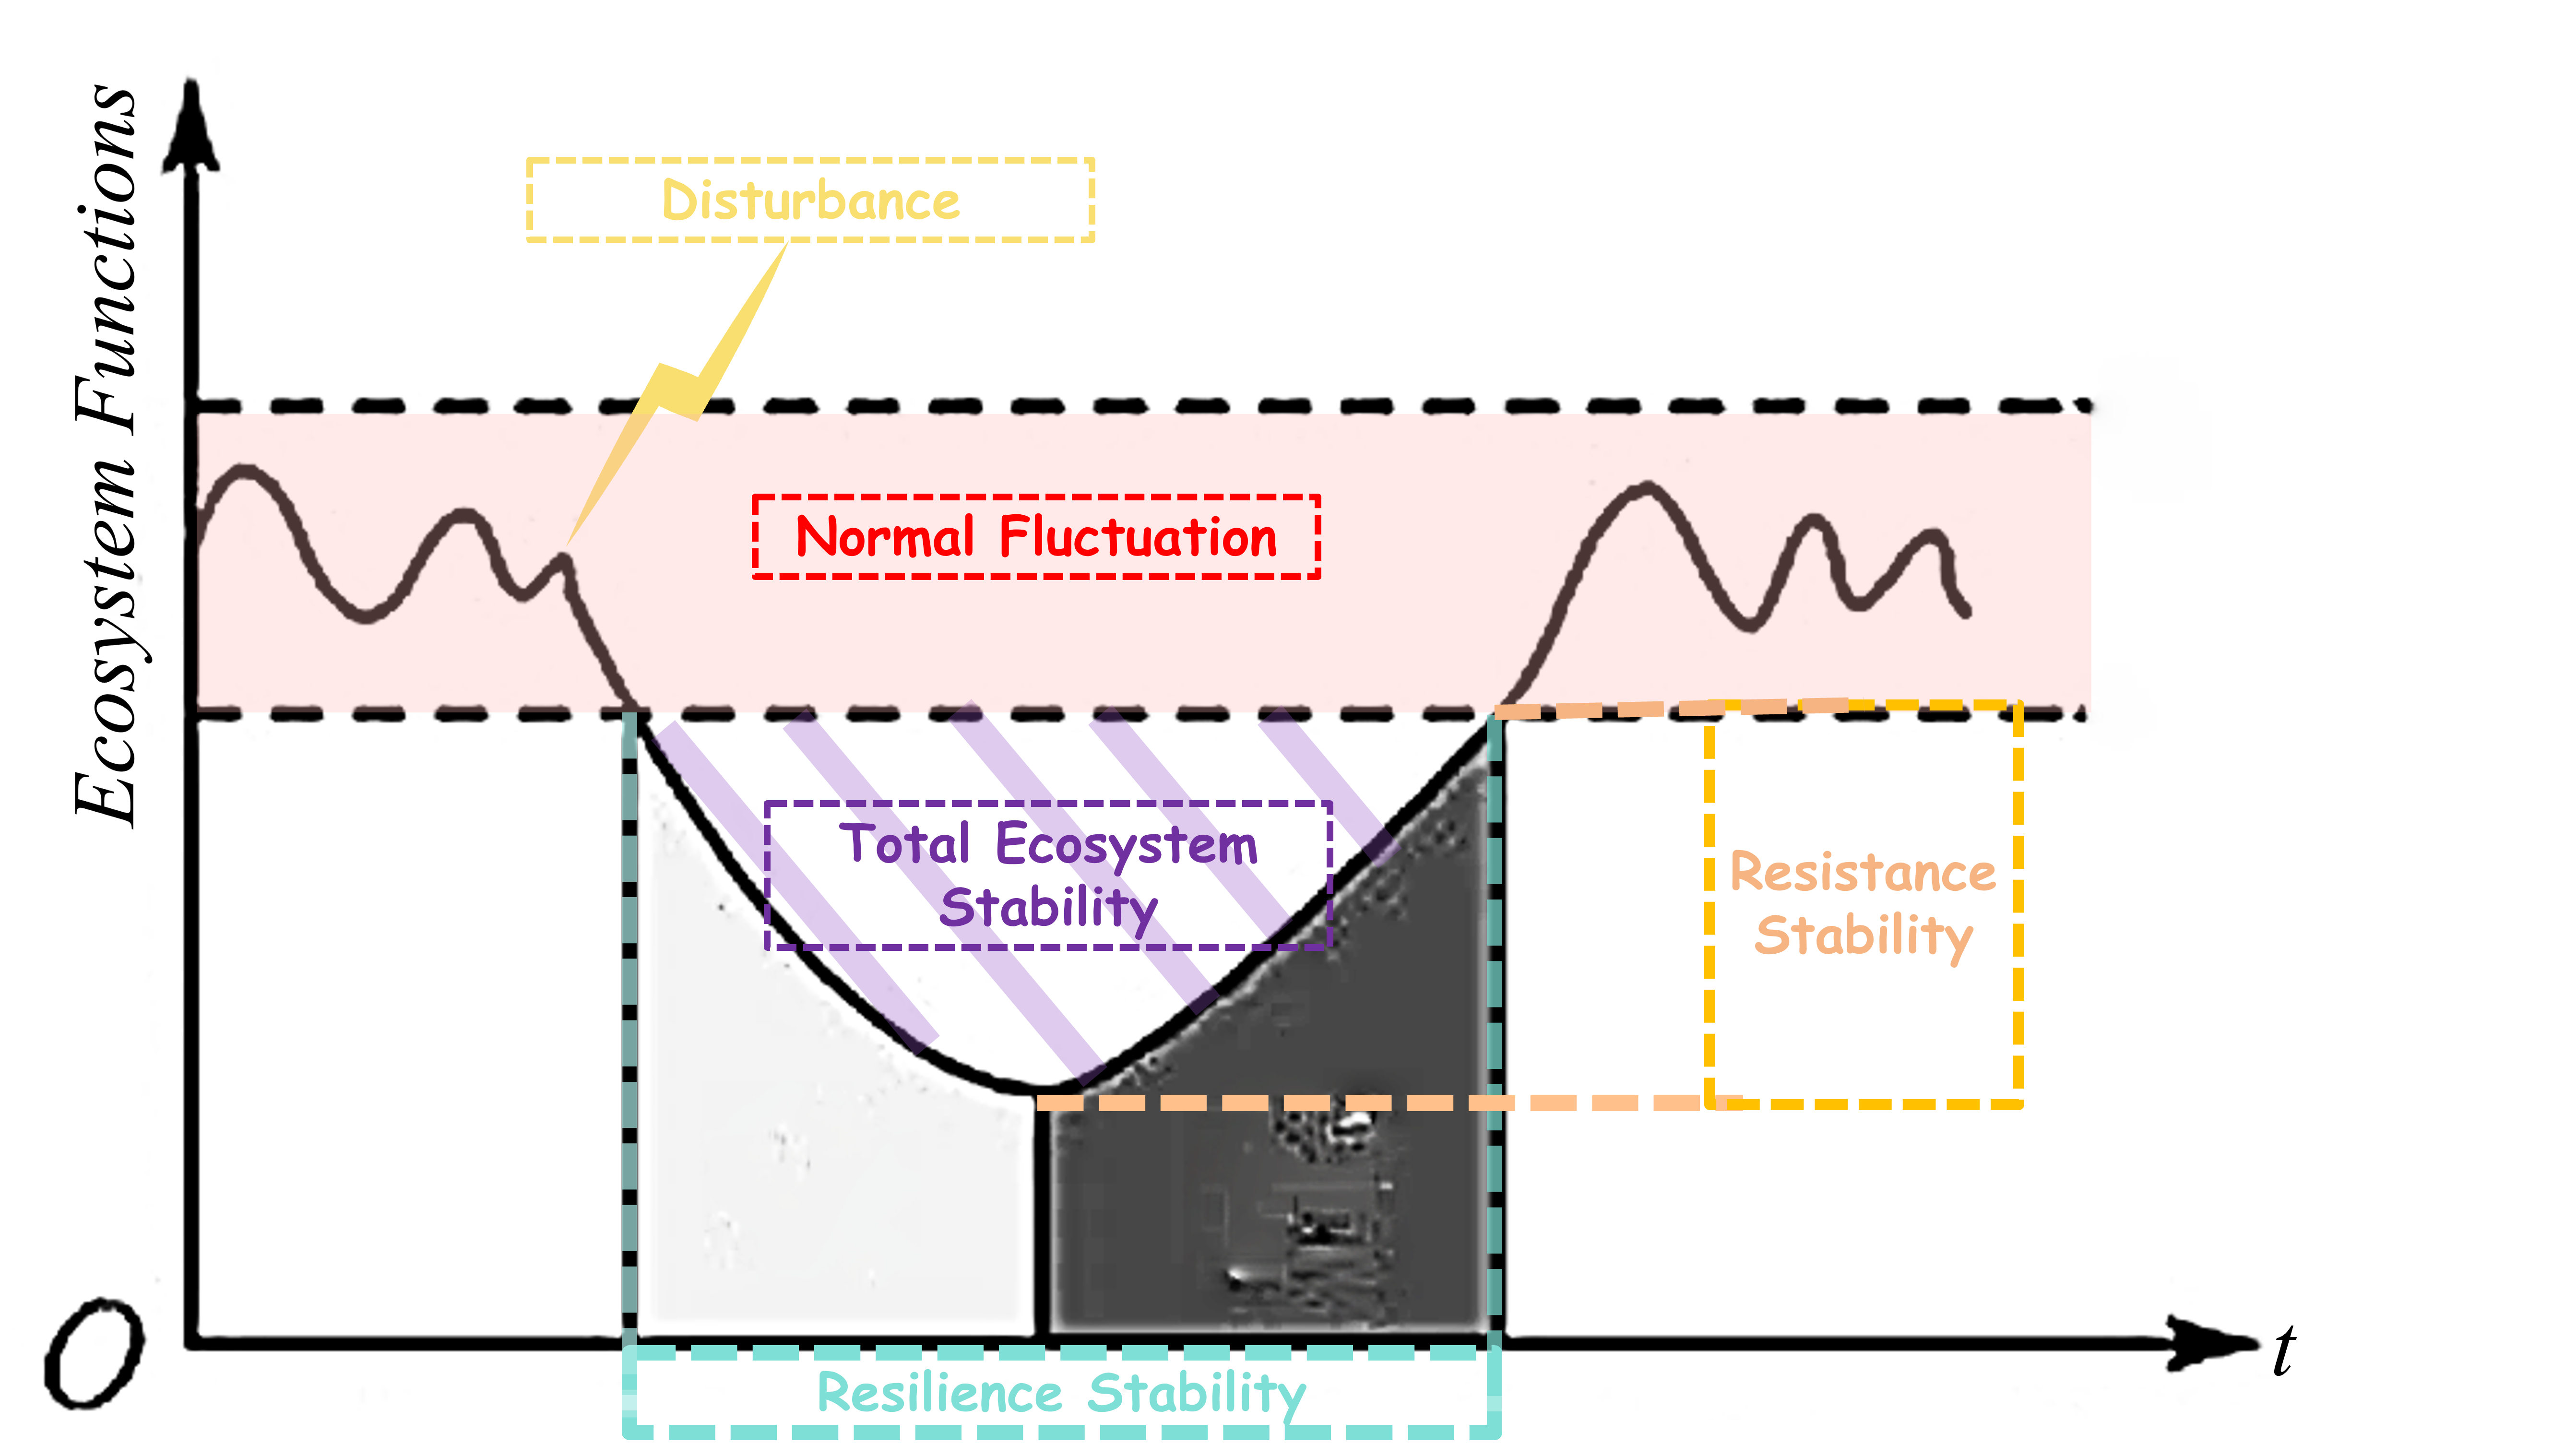
\includegraphics[width=\textwidth]{./figures/stability(task2).png}
	\caption{Ecosystem Stability Model.}
	\label{hhh}
	\end{subfigure}
	\begin{subfigure}[b]{0.44\textwidth}
		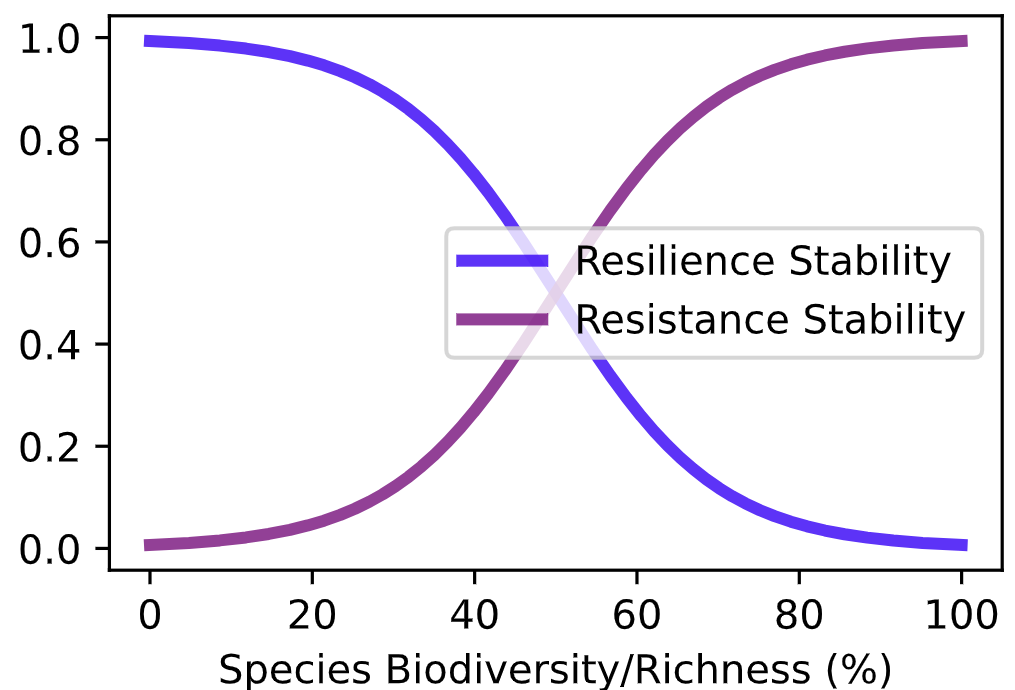
\includegraphics[width=\textwidth]{./figures/RSES(task 2).png}
	\end{subfigure}
	\caption{Illustrations of the ESM Model.}
\end{figure} 

Let a sudden disturbance occur in ecosystem (given in figure \ref{hhh}). Define $Thresh_{min}$ as the minimum threshold of functional fluctuation in a stable ecosystem, while $F$ as ecosystems' function, $t_0$ and $t_1$ respectively the first, second time when $Thresh_{min}=F$. Therefore we have:
\begin{equation}
\begin{cases}
	TES = \int_{t_0}^{t_1}(Thresh_{min}-F) \\
	RTS = Thresh_{min} - \min{F} \\
	RLS = t_1 - t_0
\end{cases},\text{and}\ \begin{cases}
	Stability \propto \frac{1}{TES} \\
	RTS \propto Richness \\
	RLS \propto \frac{1}{Richness}
\end{cases}
\label{rts}
\end{equation}

A more detailed analysis is conducted. Assign $Richness_{before}$ to represent the species richness before the reemergence of $A$ and $B$, while $Richness_{after}$ the opposite. Obviously we have: $Richness_{after}>Richness_{before}$, considering $Thresh_{min}$ as a constant, we have:
\begin{align*}
& \begin{cases}
	RTS_{after}>RTS_{before} \\
	RLS_{after}<RLS_{before} \\
\end{cases} \xrightarrow{ }\begin{cases}
	F_{after}>F_{before} \\
	(t_1-t_0)_{after}<(t_1-t_0)_{before}
\end{cases}\xrightarrow{ }TES_{after}<TES_{before} \\
&\xrightarrow{ } Stability_{after}>Stablity_{before}
\end{align*}

Therefore, we reach to the conclusion that reemergence of species $A$ and $B$ improved the overall stability of mature agricultural ecosystem. Additionally, our model explains the inner mechanism on detailed processes of how native species migrate during different evolution stages, offering new insights into animal-behavior-related ecosystem researches.

\section{Removal of Herbicides---`` \textit{No More Chemicals!} ''}
\subsection{A Stabilized Ecosystem}
\subsubsection{Higher Richness}


We further visualize the impacts of herbicides (and other chemical substances) removal by recalculating total species richness and aforementioned metrics referring to equation \ref{shiboqi_hetiban}. Results are shown in figure \ref{sbq}. From figure \ref{tk} it can be concluded that, loss of species richness triggered by overuse of chemicals are mitigated but still having negative effects on ecosystem stability, while figure \ref{2} demonstrates that herbicide removal could directly contribute to higher biodiversity and stability, where the minimum value has been elevated to 19.8\%.
\begin{figure}[h]
	\centering
	\begin{subfigure}{\textwidth}
	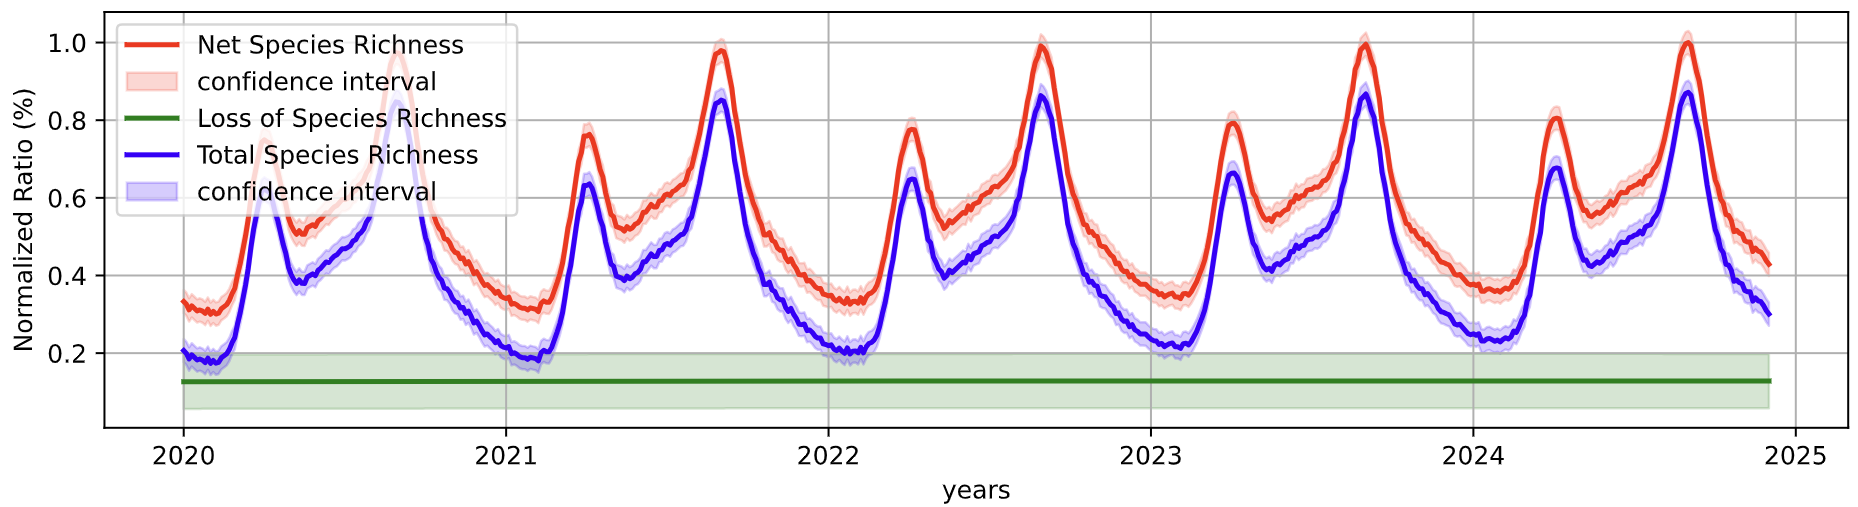
\includegraphics[width=\textwidth]{./figures/shiboqi_hetiban(task3).png}
	\caption{Net \& Total Species Richness when herbicides are removed}
	\label{tk}
	\end{subfigure}
	\begin{subfigure}{\textwidth}
		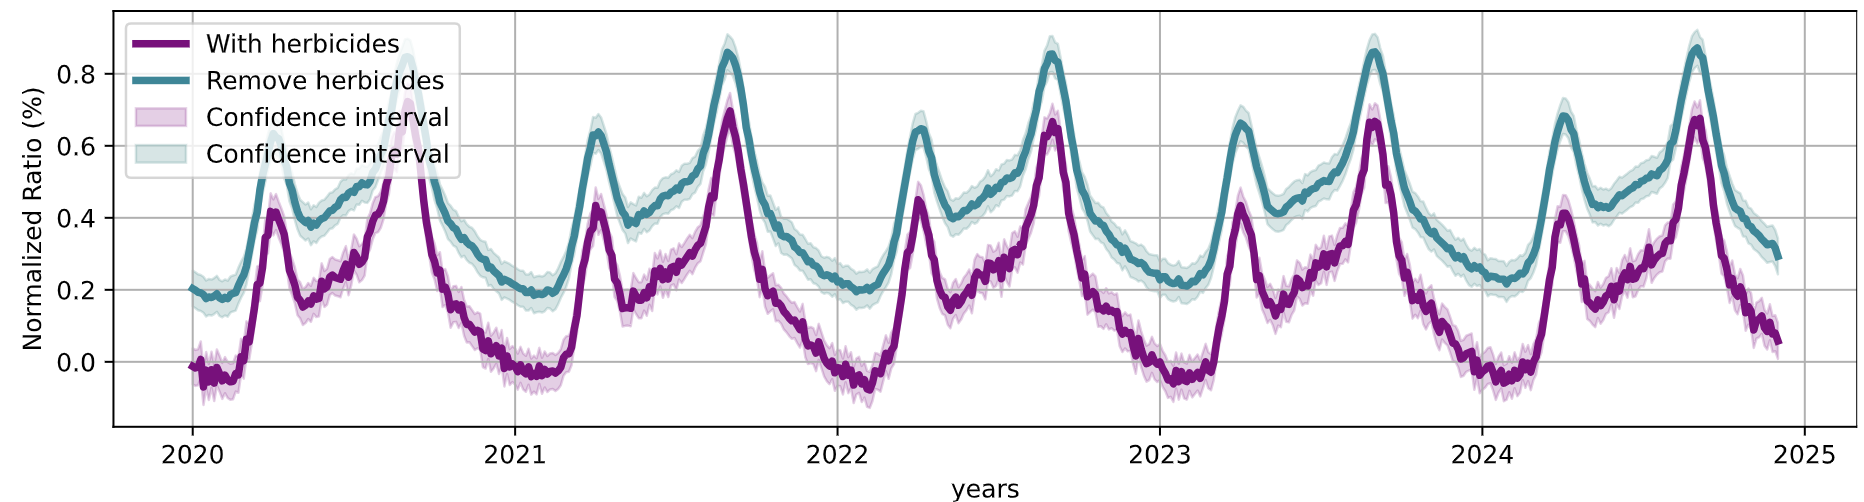
\includegraphics[width=\textwidth]{./figures/shiboqi_Task3(1).png}
		\caption{Comparisons on total species richness before and after herbicides' removal.}
		\label{2}
	\end{subfigure}
	\caption{Effects of herbicide removal on ecosystem stability and species richness.}
	\label{sbq}
\end{figure}
\subsubsection{Stronger Resistance}
According to equation \ref{rts}, we conclude that biodiversity and species richness is positively proportional to ecosystem stability. Additionally, in equation \ref{modified} we optimize formula \ref{original} and infer the removal of herbicides positively facilitates biomass and biodiversity of either producers or consumers, indicating an increase in resistance stability and a decrease in resilience stability, as is illustrated in figure \ref{resistance}

\begin{figure}
	\centering
	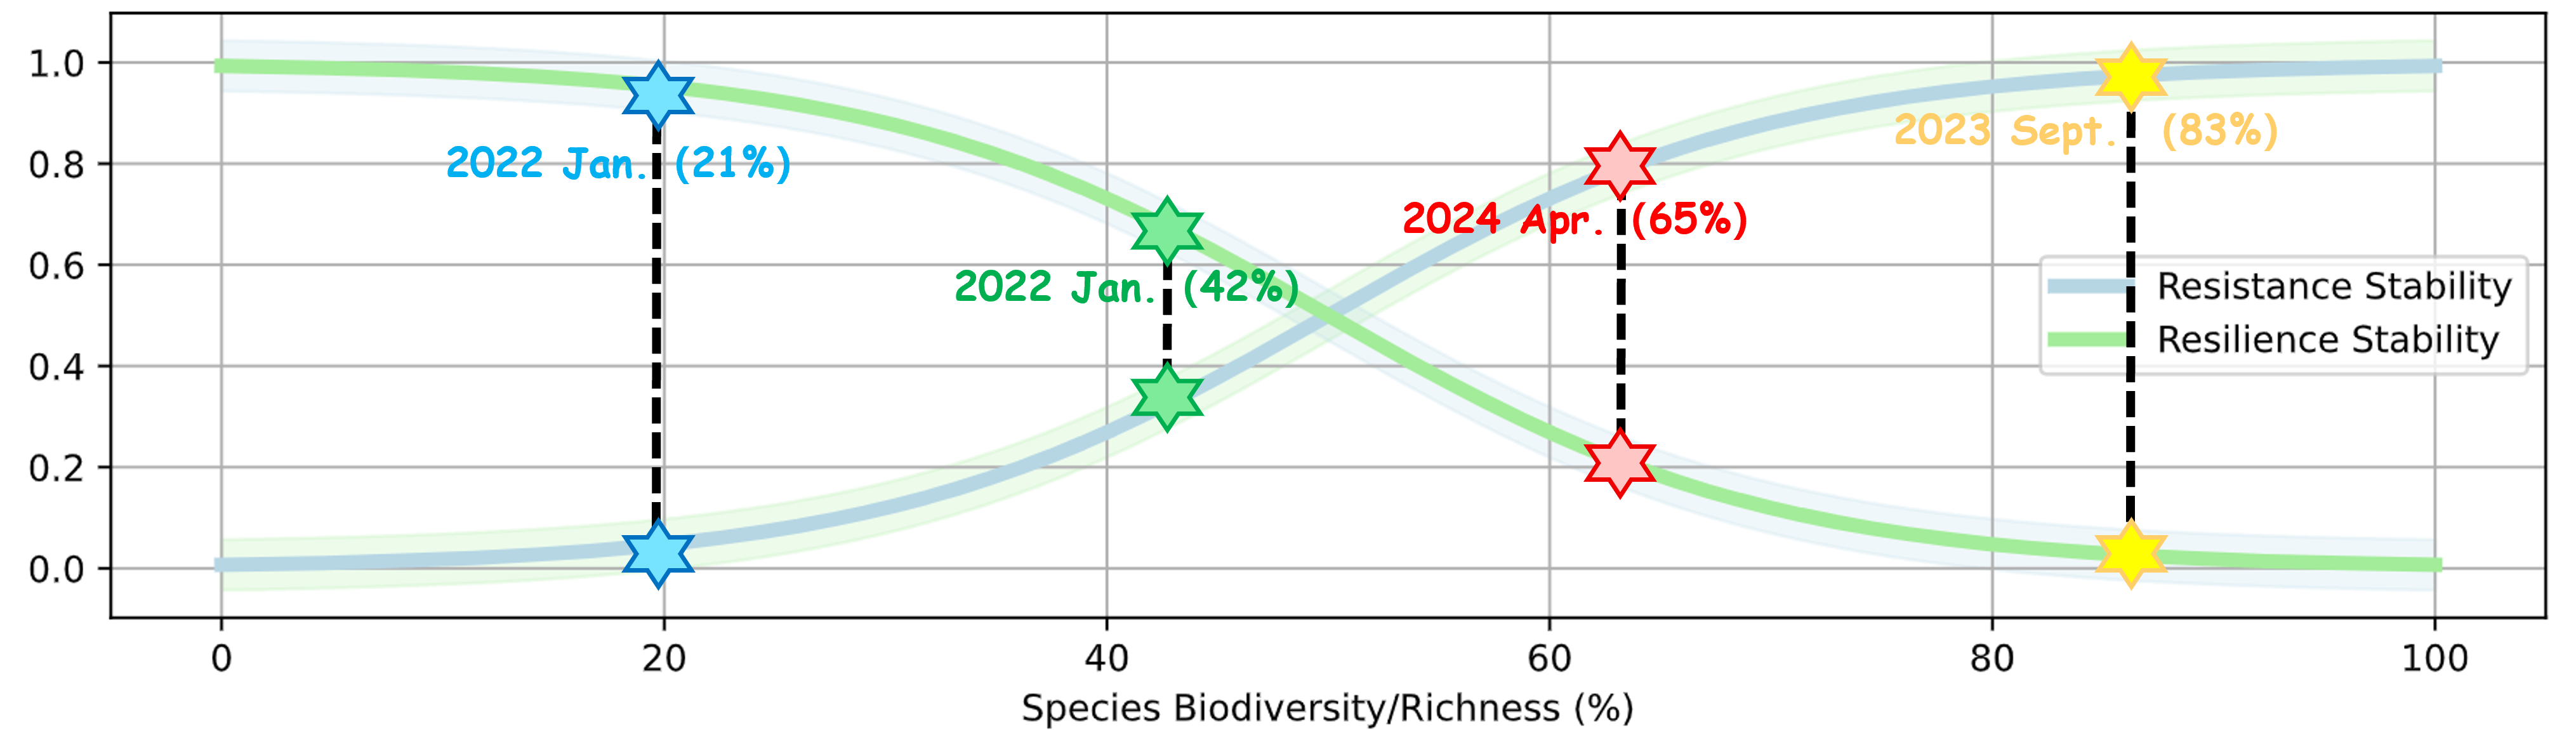
\includegraphics[width=0.8\textwidth]{./figures/resistance(task3).png}
	\caption{$RTS$ and $RLS$ when herbicide are removed.}
	\label{resistance}
\end{figure}

Similar to the stability analysis conducted in section 5.2, let footnote $IH$ stands for ``Including Herbicide'' and $EH$ for ``Excluding Herbicide'', from figure \ref{sbq} and \ref{resistance} obviously we have:$$
\begin{cases}
	RTS_{EH}>RTS_{IH} \\
	RLS_{EH}<RLS_{IH}
\end{cases}\xrightarrow{ }\begin{cases}
	F_{EH}>F_{IH} \\
	(t_1-t_0)_{EH}<(t_1-t_0)_{IH}
\end{cases}\xrightarrow{ }TES_{EH}<TES_{IH}
\xrightarrow{ }Stability_{EH}>Stability_{IH}
$$

Therefore, we reach to the conclusion that: When herbicide is removed, the ecosystem will become more stable. The deeper mechanism can be explained from two perspectives. On the one hand, removal of herbicide and other chemicals reduce the loss of species richness by nourishing consumers and predators in food web, which in turn contributes to a higher biodiversity and system stability; On the other hand, removal of herbicide increases resistance stability and decreases resilience stability, which leads to an elevation in overall ecosystem stability.
\subsection{Introduction of bats}
%%%%%%%%%% 正文结束 %%%%%%%%%%%%
%%%%%%%%% 参考文献开始 %%%%%%%%%%%%
\newpage
\begin{thebibliography}{00}
	
\bibitem{1} % 第一个参考文献，以此类推
	
	
\bibitem{2} % 第二个参考文献
	
	
\bibitem{3} % 第二个参考文献
	
\end{thebibliography}
%%%%%%%%% 参考文献结束 %%%%%%%%%
%%%%%%%%% 全文结束 %%%%%%%%%%%%%
\end{document}
\end
